\chapter{Sequenzdiagramme}
Um die verschiedenen möglichen Abläufe zu verdeutlichen wurden einige Sequenzdiagramme erstellt, die die Funktionen der Anwendung einfach und effektiv erklären.

\begin{itemize}

    \begin{figure}[H]
        \centering
        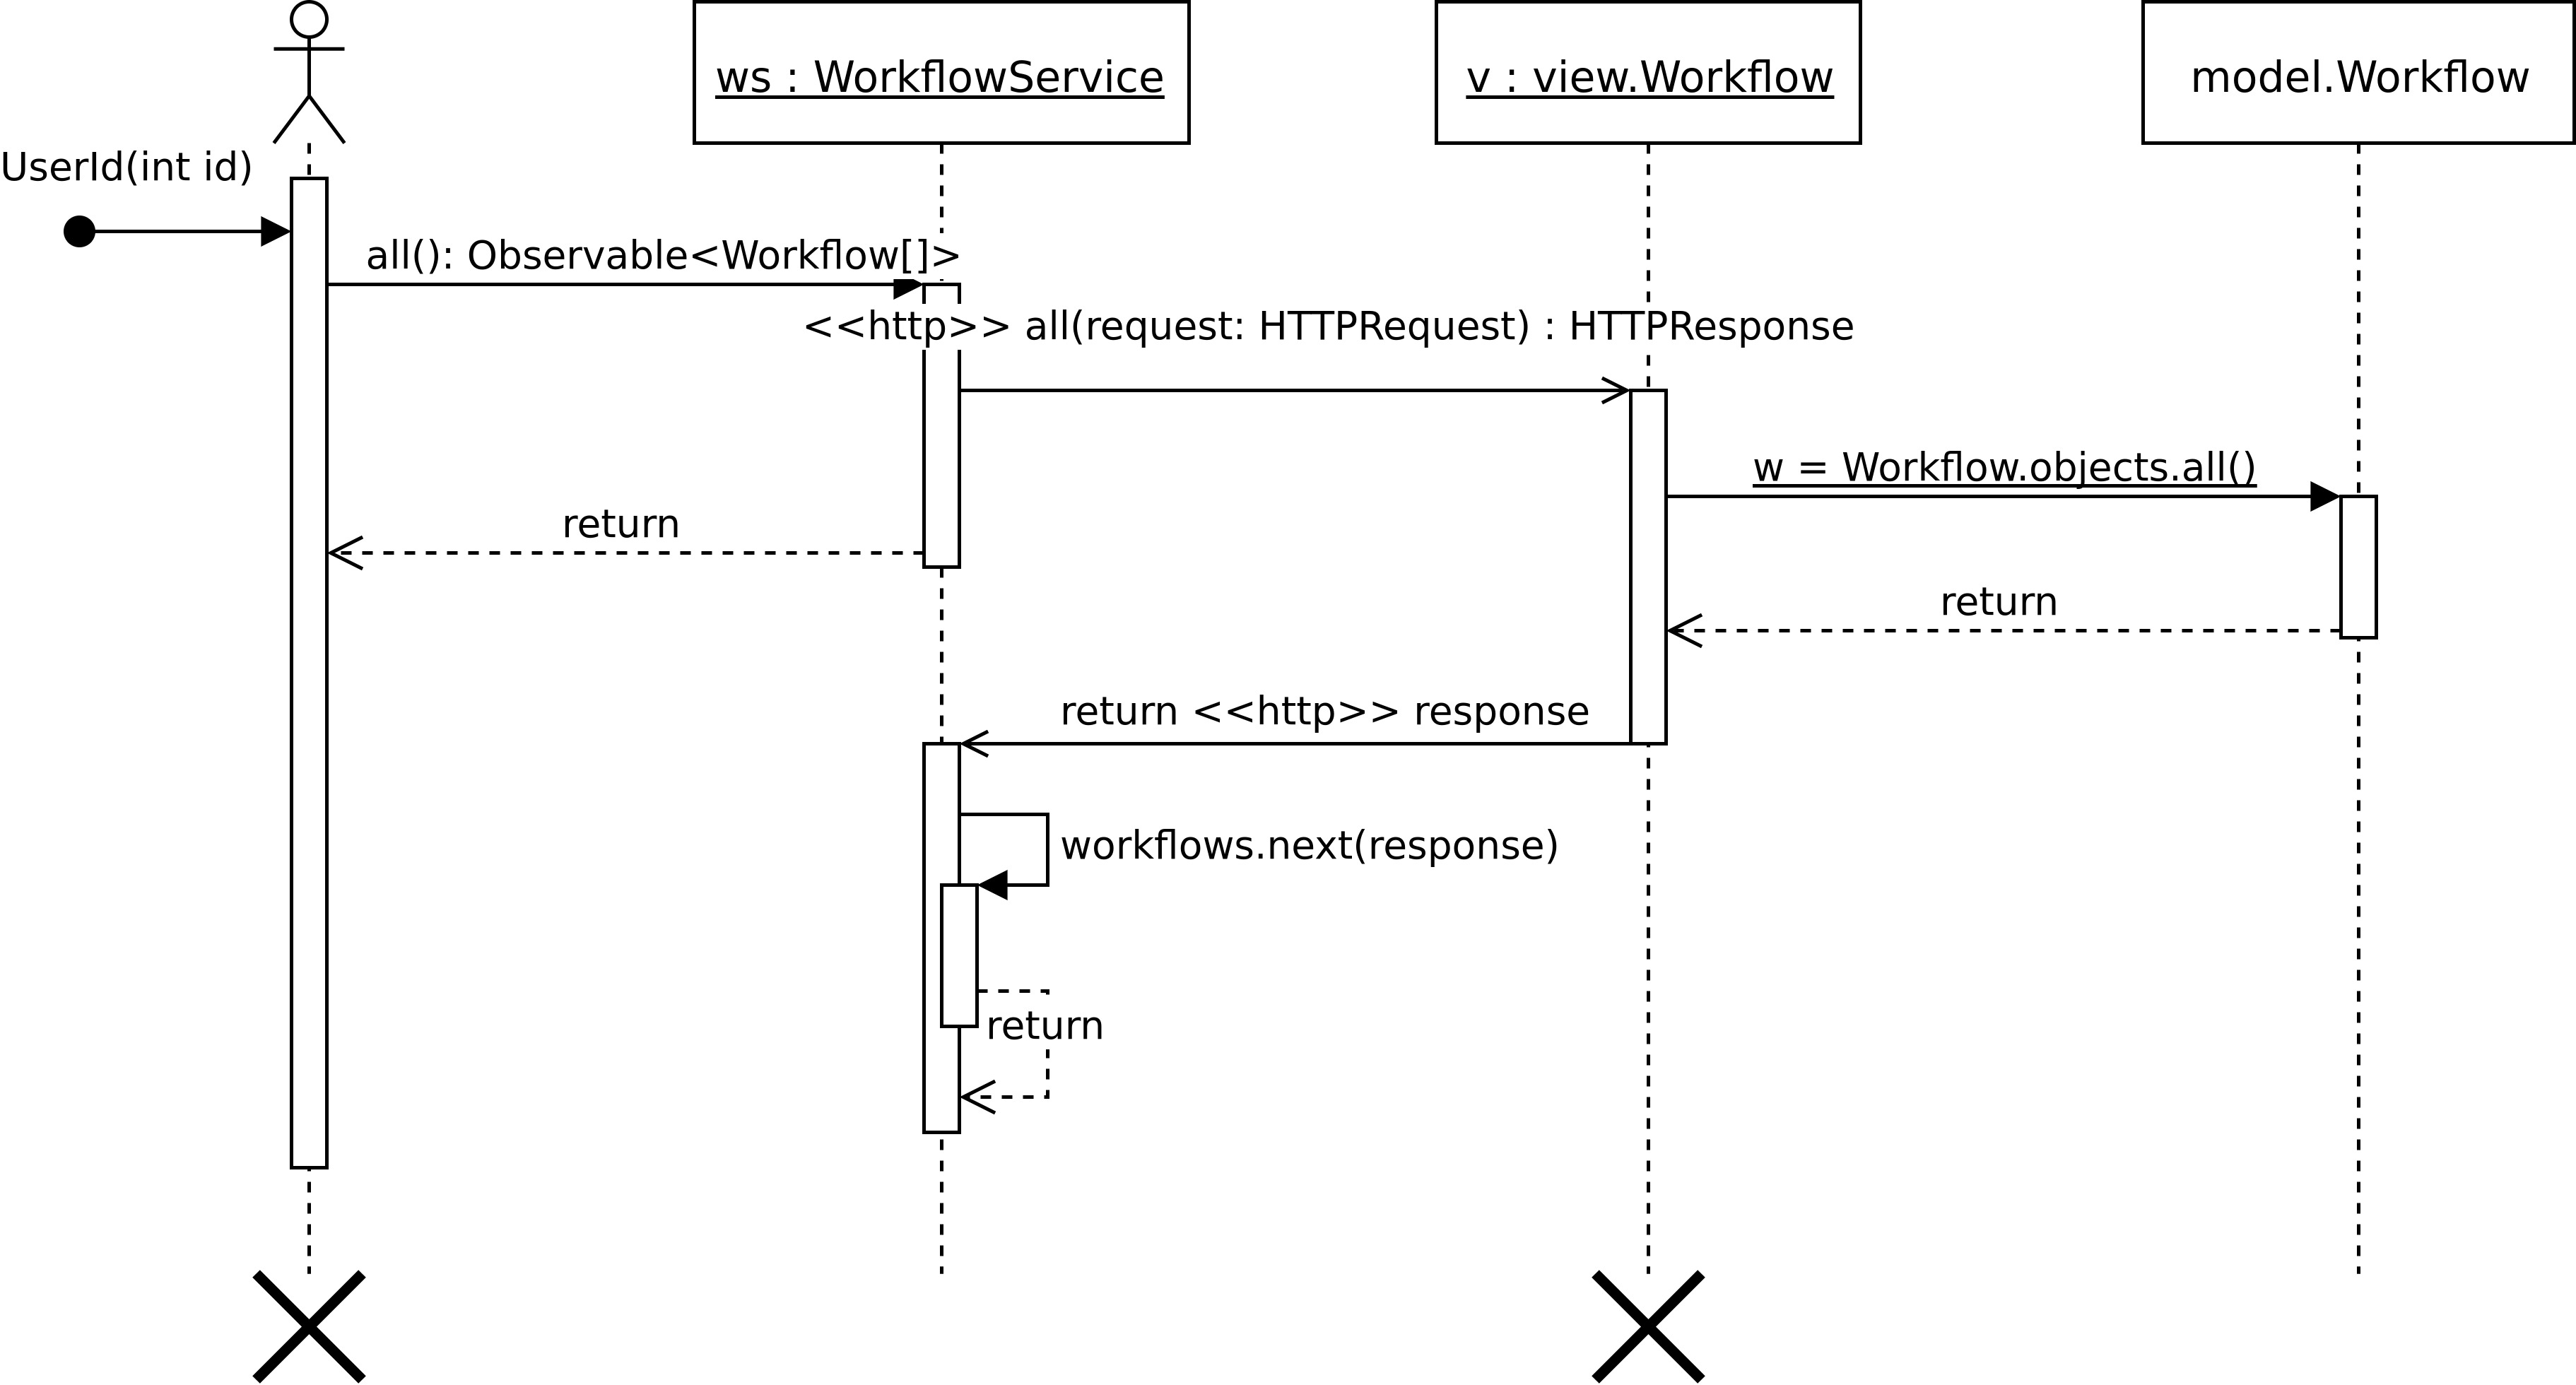
\includegraphics[width=15cm]{images/sqd_get_all_workflows.jpg}
        \caption{Get All Workflows}
        \label{sqd_get_all_workflows}
    \end{figure}

    \item Der Benutzer ist mit seiner eindeutigen User ID angemeldet und will alle seine Workflows sehen (Abbildung \ref{sqd_get_all_workflows}). Hierfür wird clientseitig eine Liste an Observables in einer Instanz von WorkflowService angelegt. Dann wird ein HTTP Request an die zugehörige serverseitige Instanz von view.Workflow geschickt. Diese frägt bei der Datenbank in model.Workflow die Daten an und schickt sie per HTTP Response zurück an die vorherige Instanz von WorkflowService. Hier wird anschließend die Referenz auf die Observables aktualisiert, wodurch der Benutzer jetzt alle seine Workflows angezeigt bekommt. \newline\newline
    
    \begin{figure}[H]
        \centering
        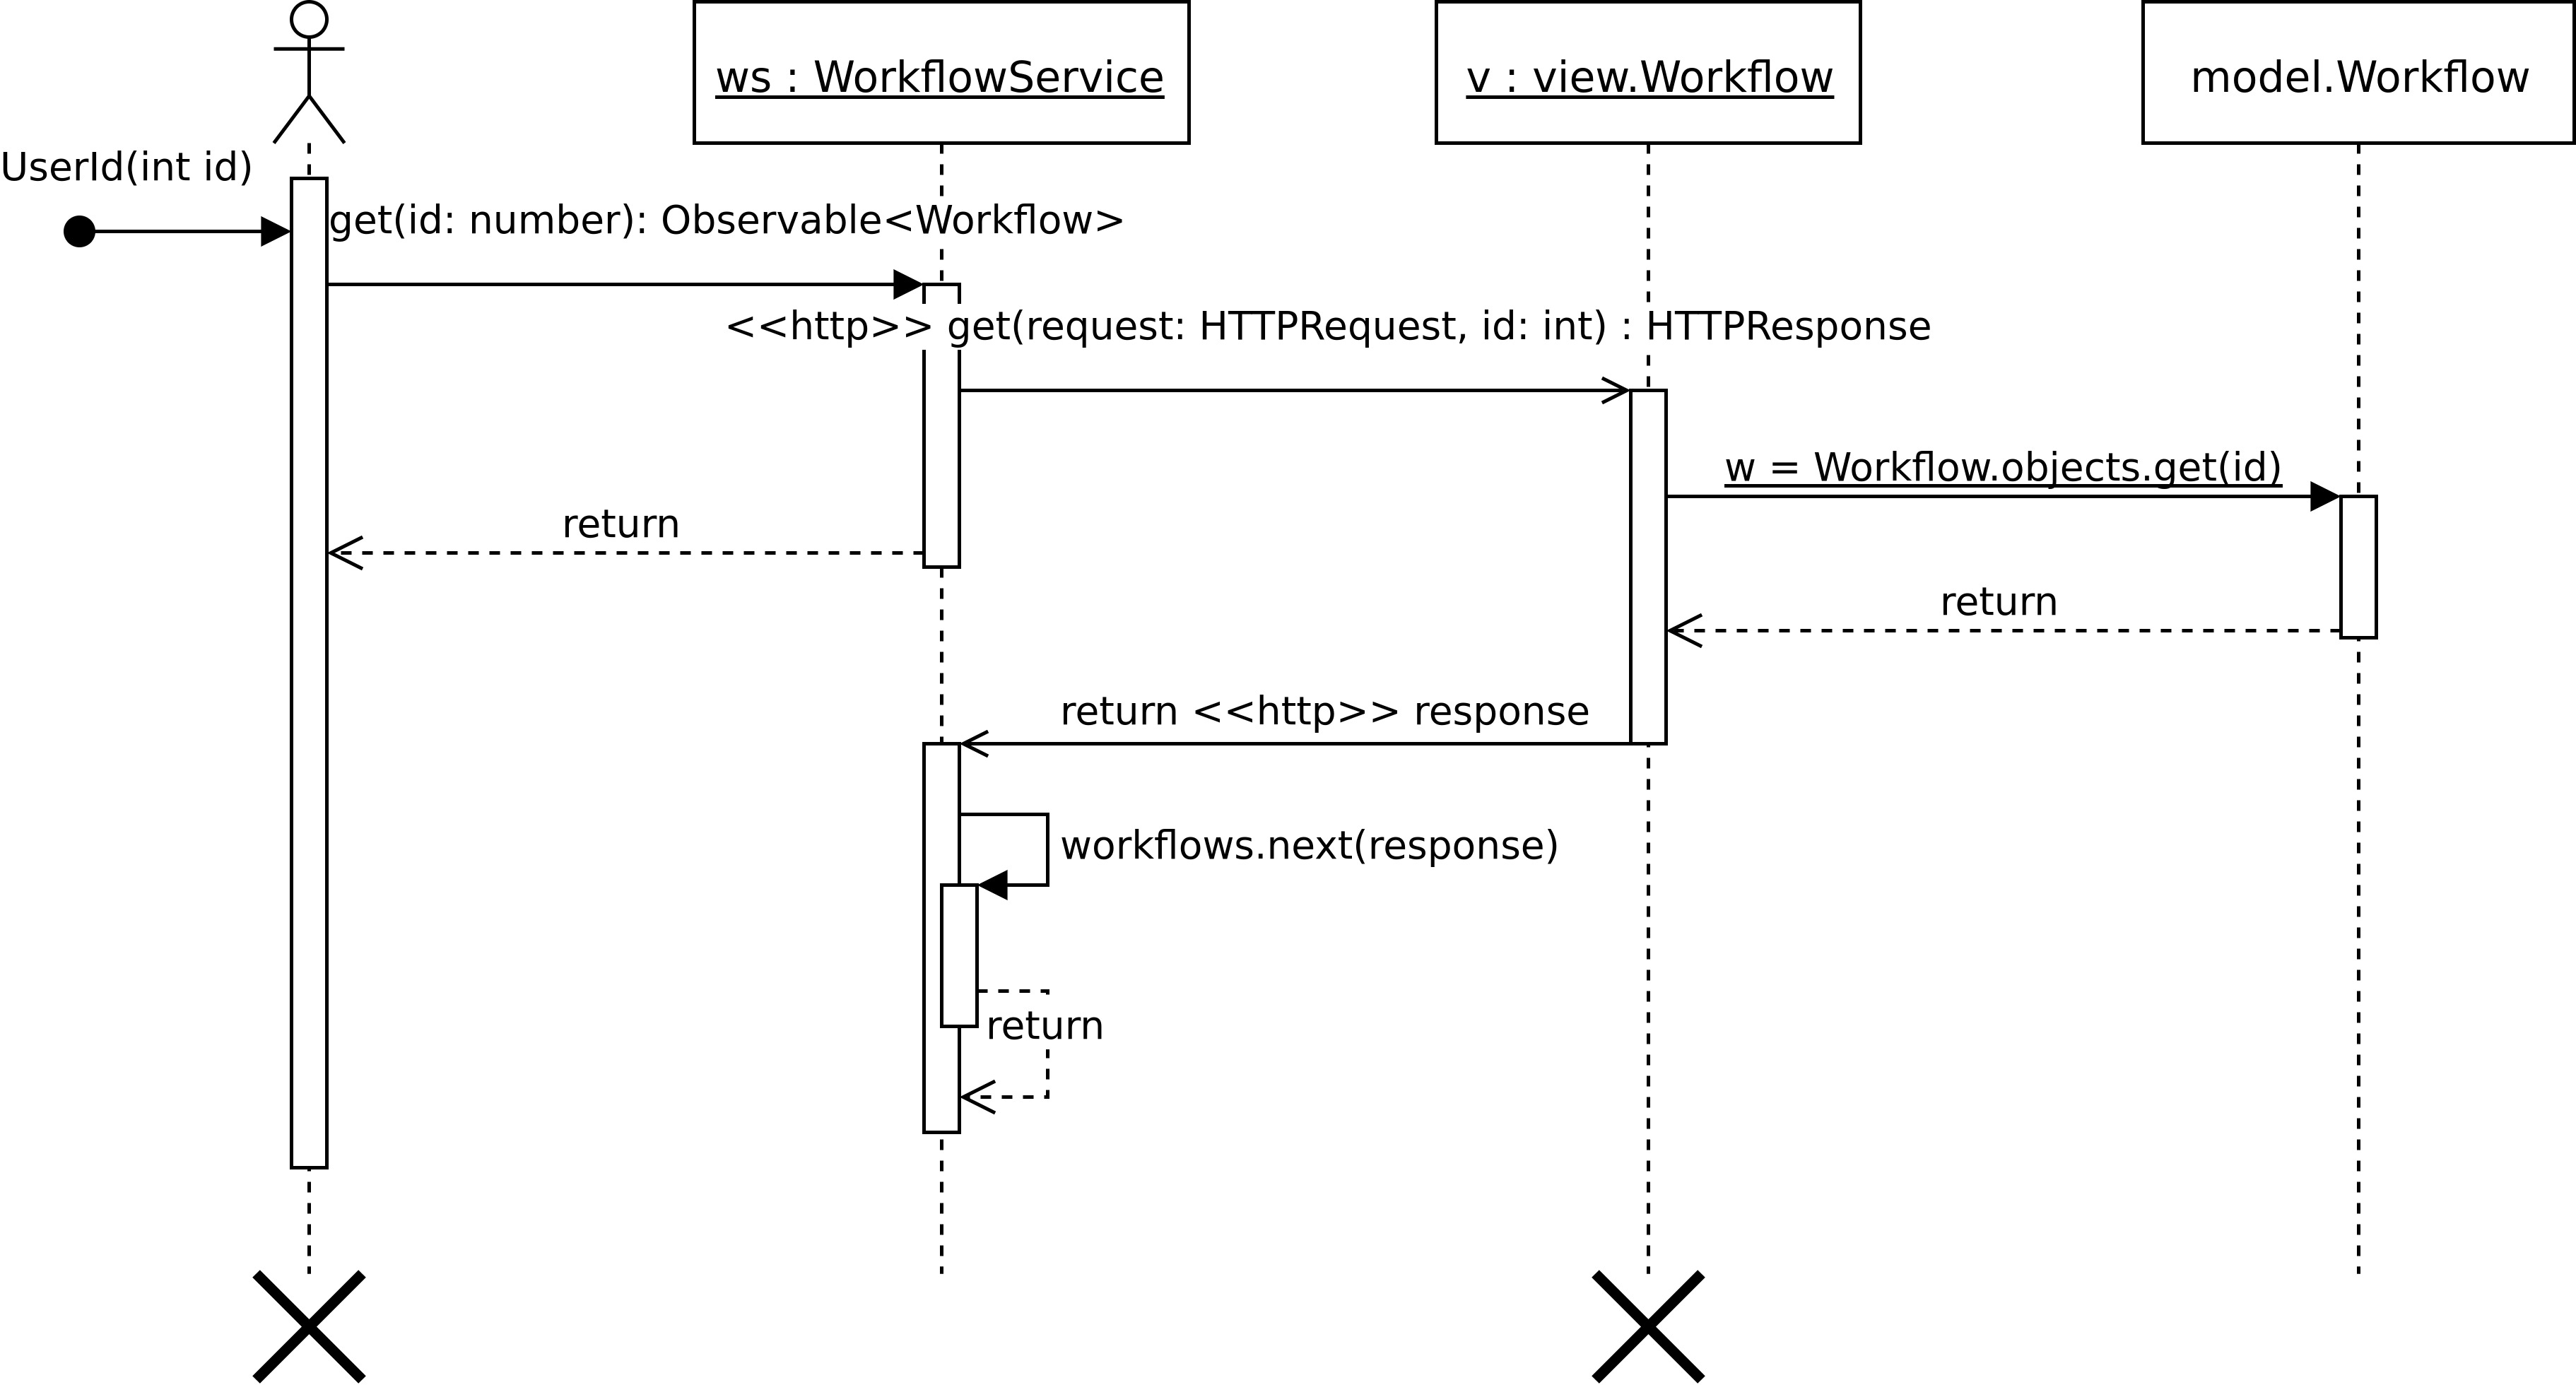
\includegraphics[width=15cm]{images/sqd_get_workflow.jpeg}
        \caption{Get Workflow}
        \label{sqd_get_workflow}
    \end{figure}
    
    \item     
    Bei Abbildung \ref{sqd_get_workflow} verläuft das analog wie bei Abbildung  \ref{sqd_get_all_workflows}, mit der Ausnahme, dass hier entsprechend immer nur ein Workflow anhand seiner ID geladen wird. Hier wird u.a. ebenfalls der aktuelle Ausführungsstatus des Workflows geladen.\newline\newline
   
    \begin{figure}[H]
        \centering
        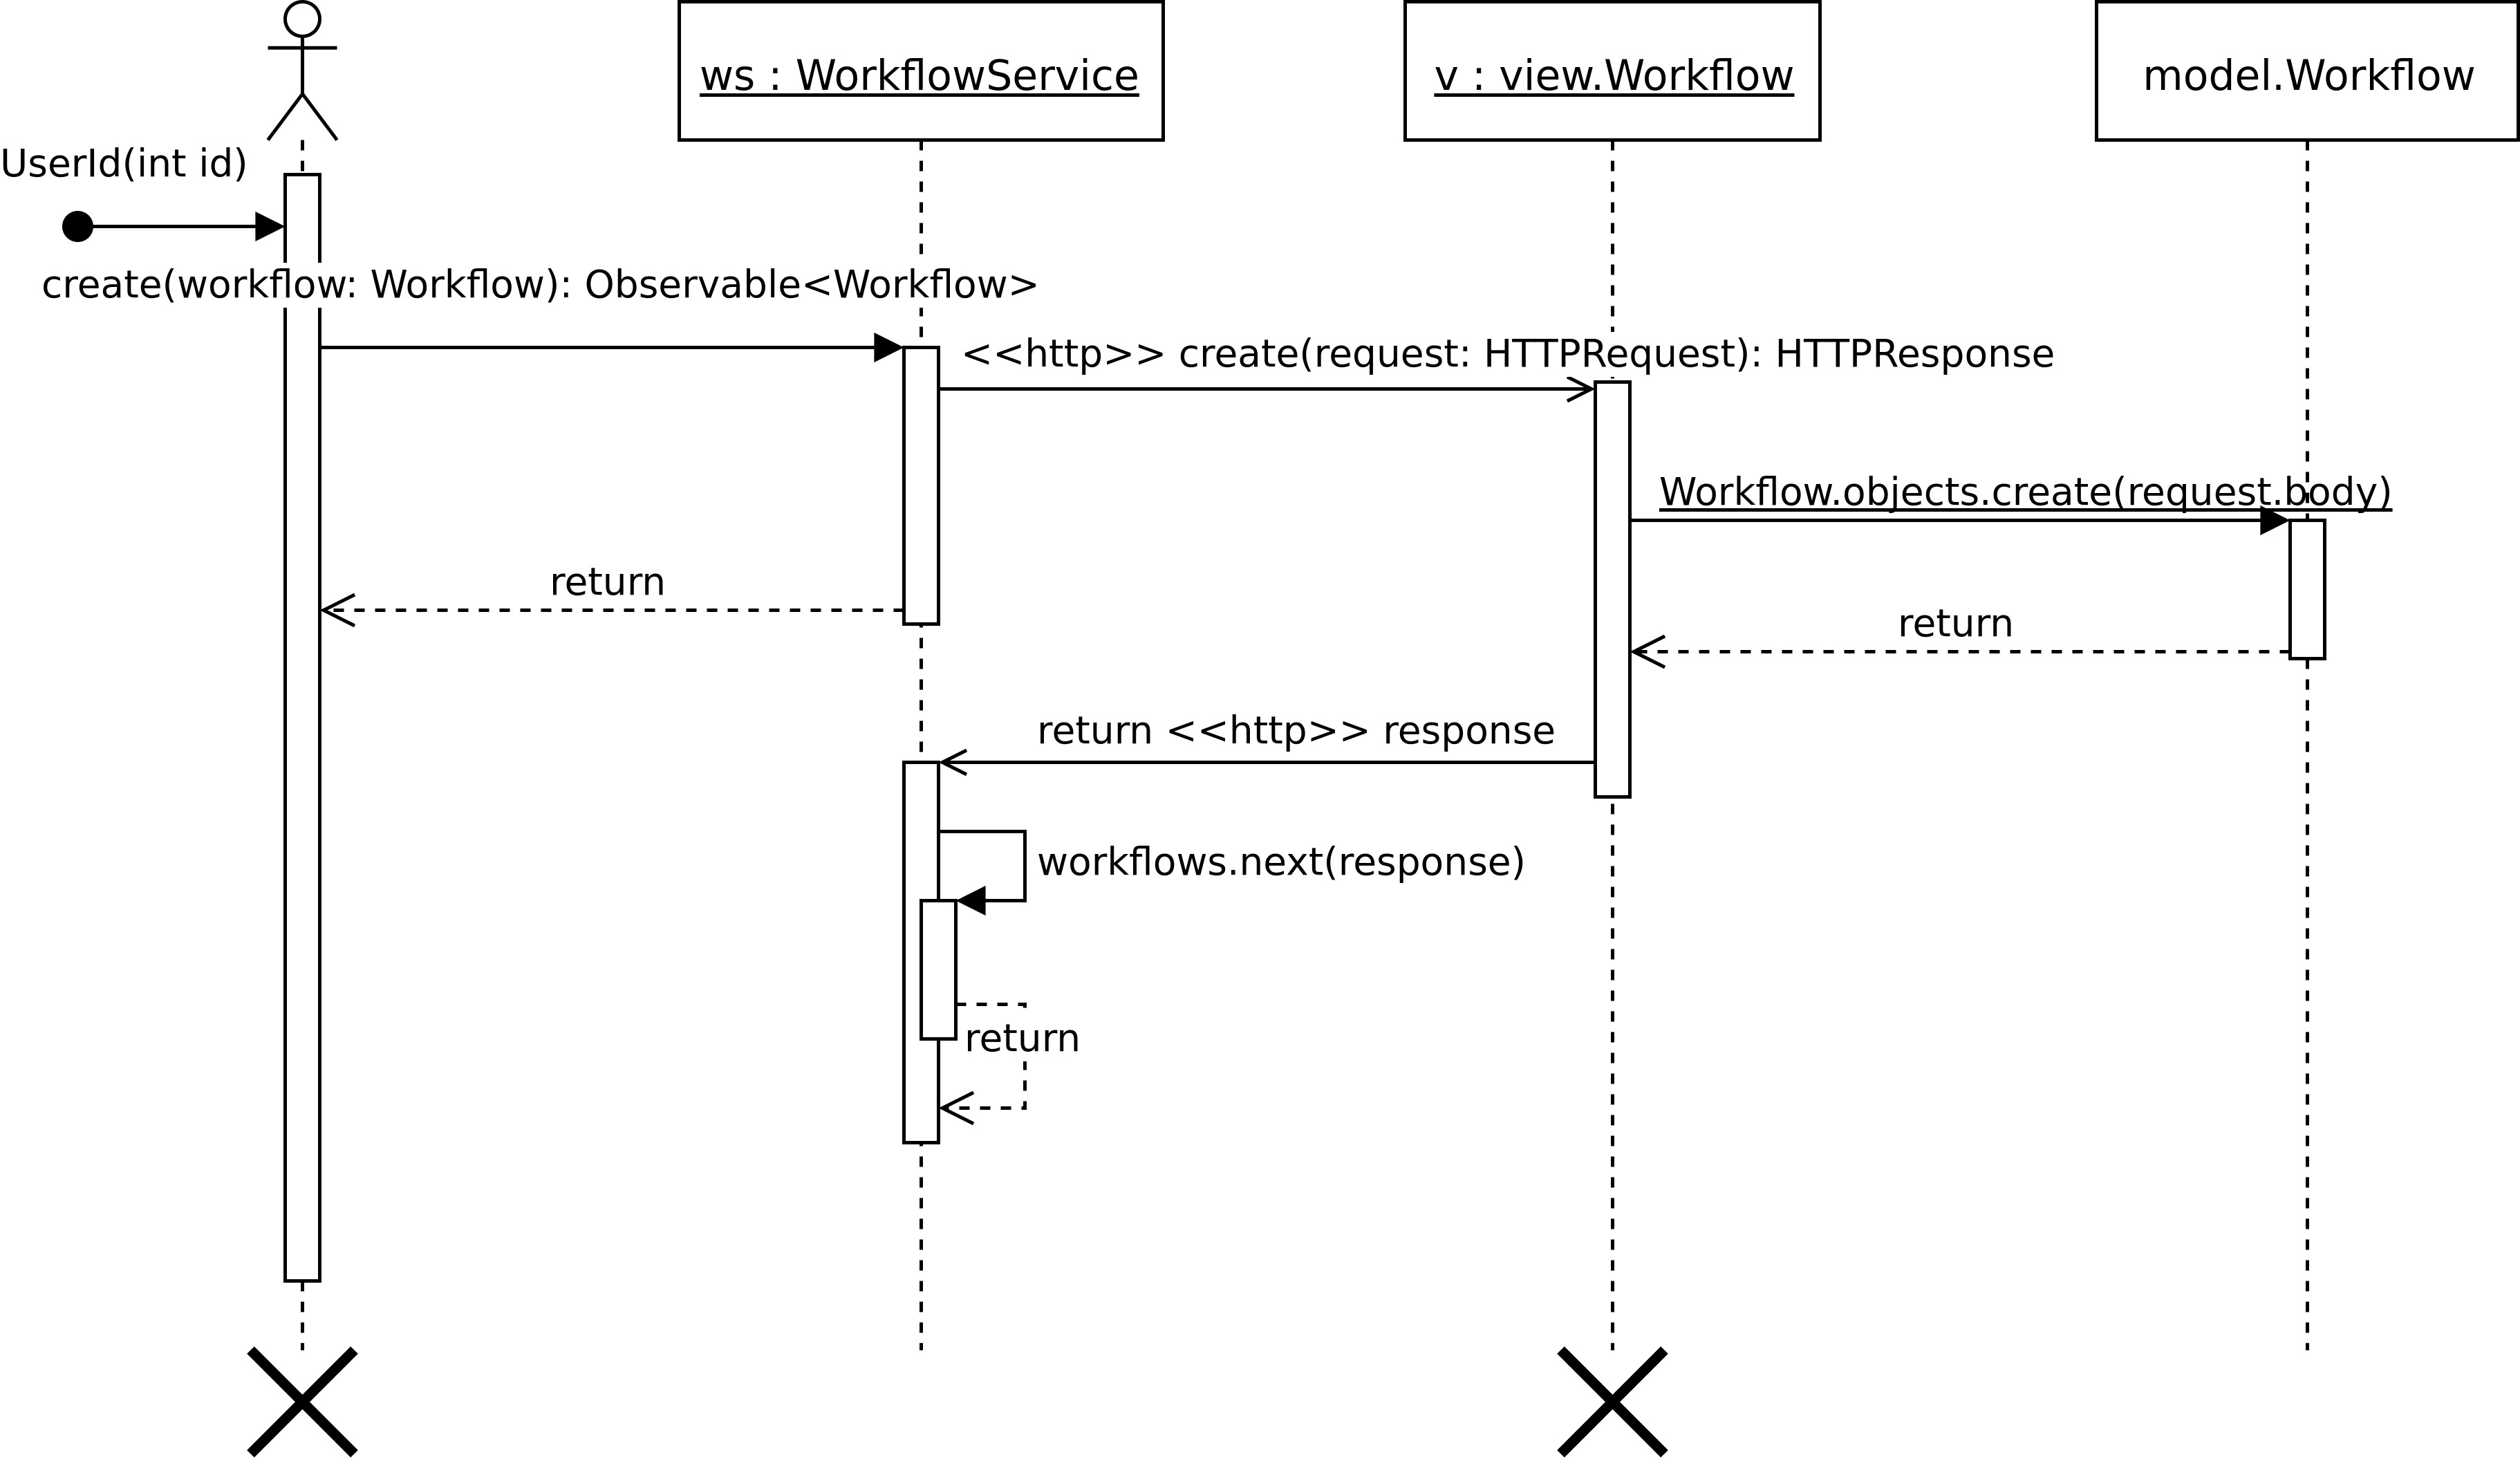
\includegraphics[width=15cm]{images/sqd_save_workflow.jpeg}
        \caption{Save Workflow / Create new Workflow}
        \label{sqd_save_workflow}
    \end{figure}

    \item Der Benutzer ist bereits mit seiner eindeutigen User ID eingeloggt und hat einen Workflow geladen. Der Benutzer will den Workflow als neuen Workflow speichern (Abbildung \ref{sqd_save_workflow}). Er drückt auf \grqq{}speichern\grqq{}, hier wird er aus dem Editor auf WorkflowService mittels der create(workflow) Methode geleitet. Diese sendet einen HTTP Request an view.Workflow. Hier wird dann serverseitig ein neuer Workflow in der Datenbank angelegt. Danach gibt es einen HTTP Response zurück zum WorkflowService. Dies geht analog um einen neuen leeren Workflow zu kreieren, nur das hierbei nicht ein bereits vorhandener Workflow gespeichert oder gar geladen sein muss. \newline\newline
    
    \begin{figure}[H]
        \centering
        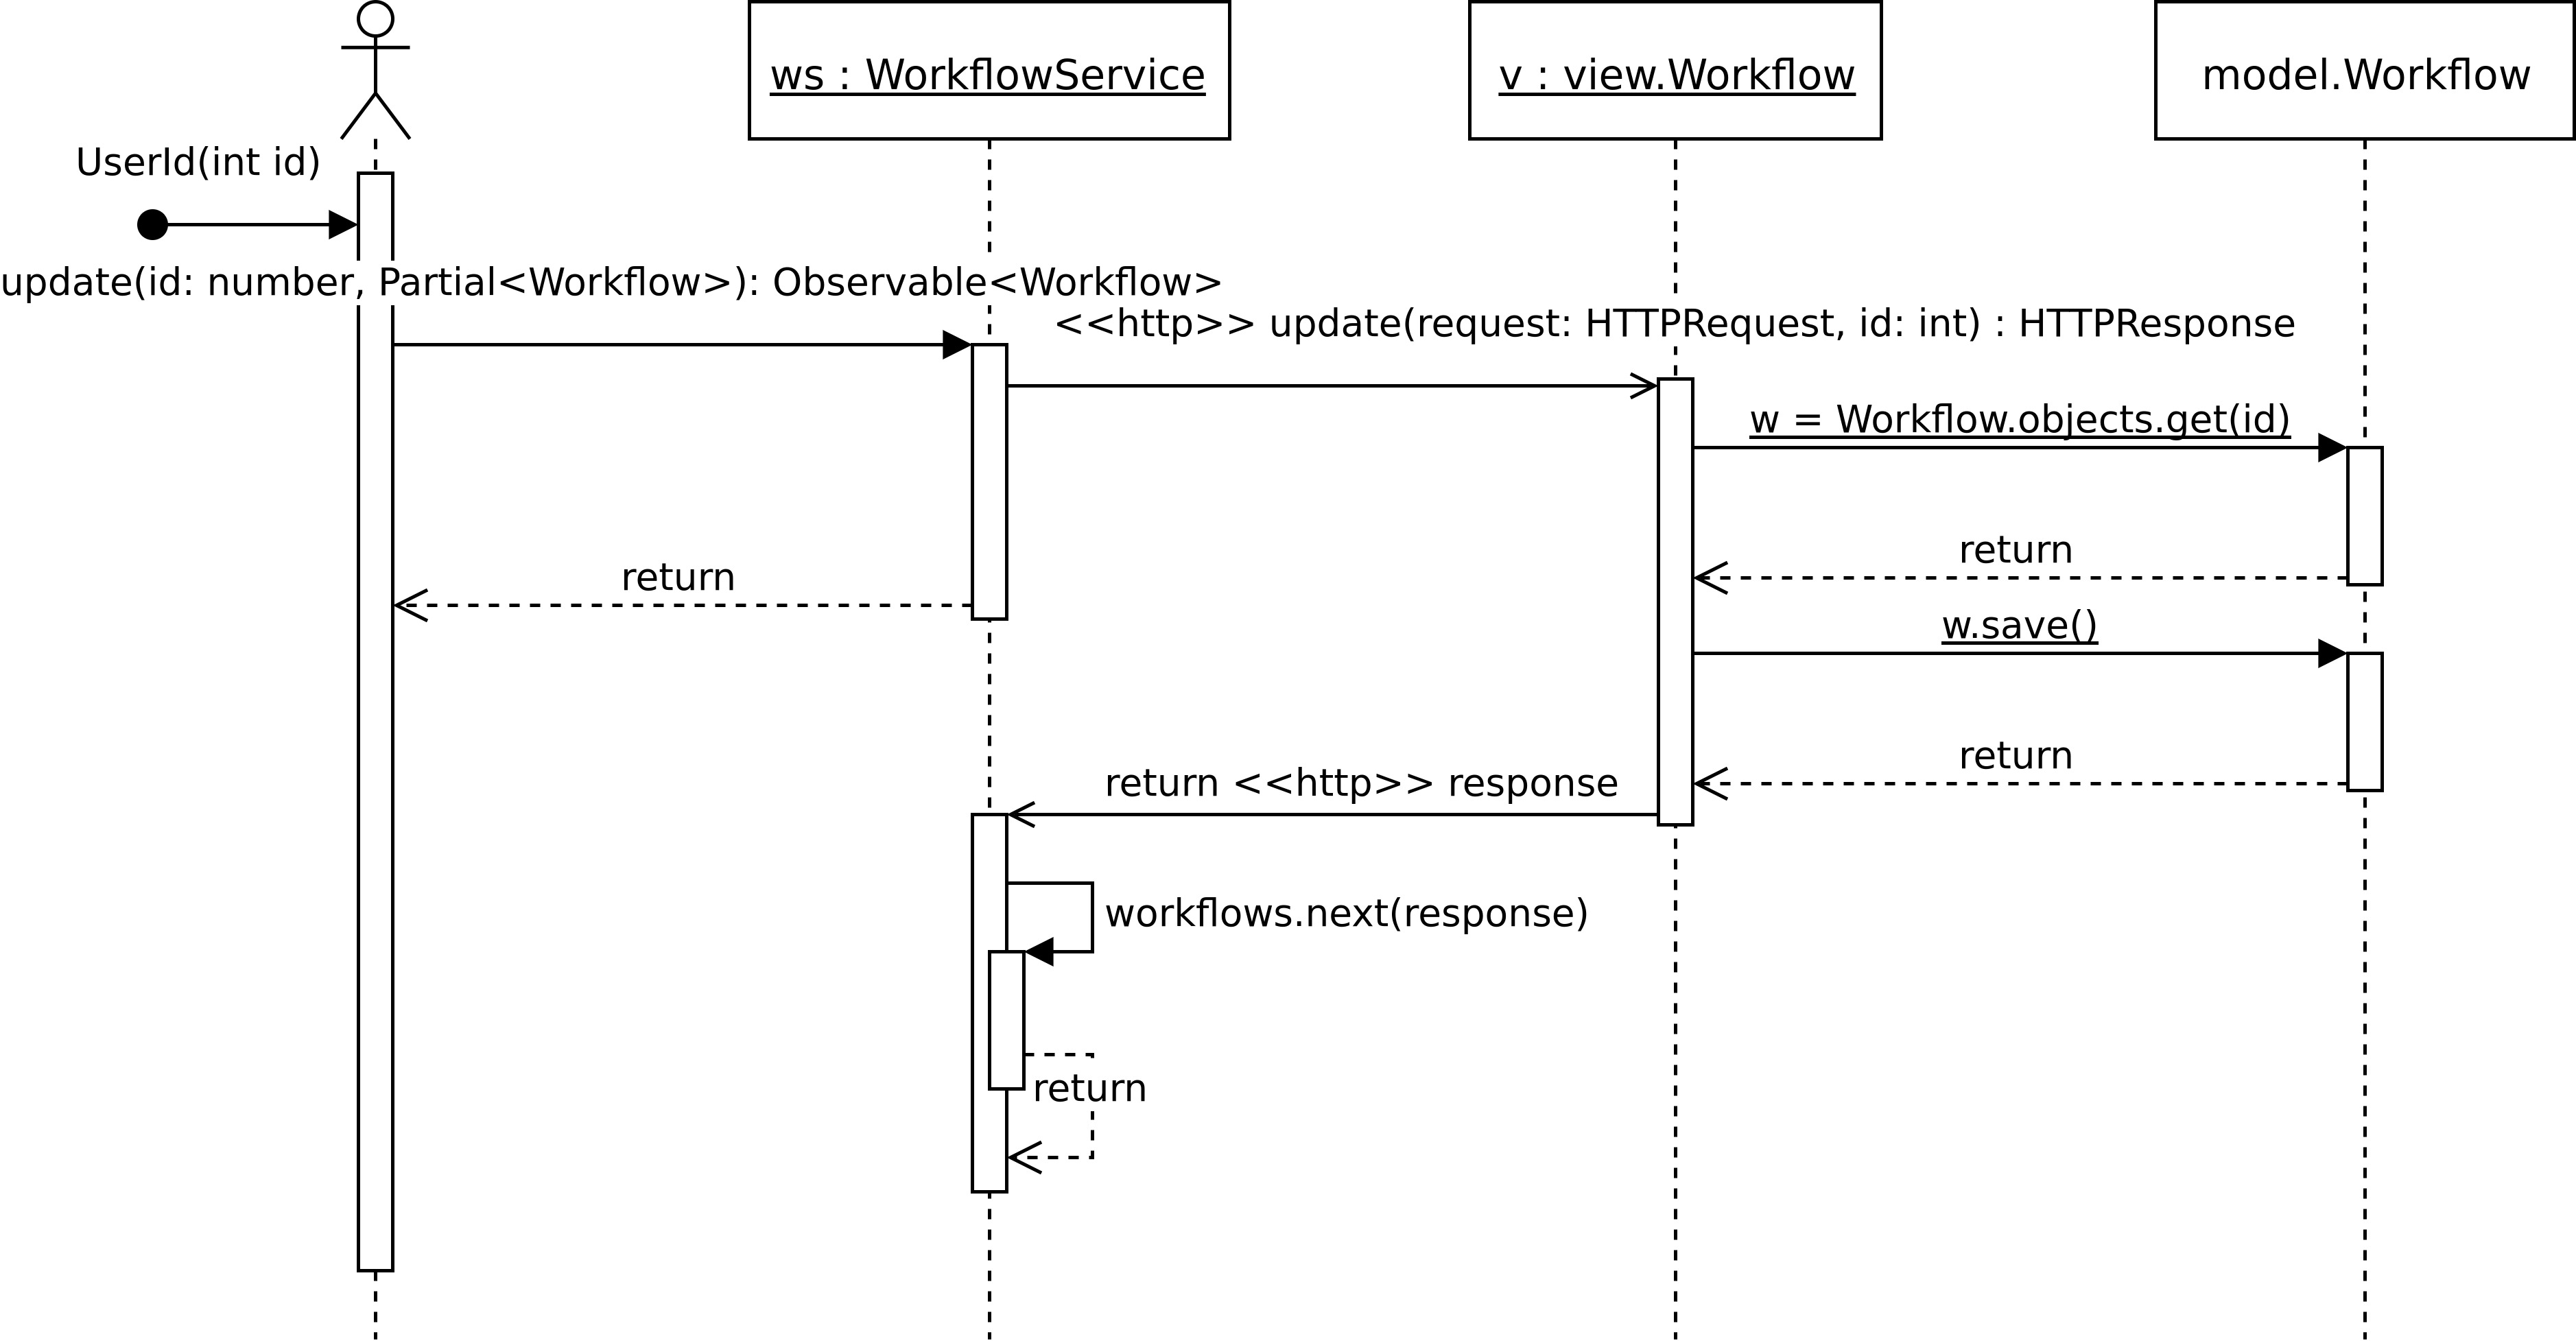
\includegraphics[width=15cm]{images/sqd_edit_workflow.jpg}
        \caption{Edit Workflow}
        \label{sqd_edit_workflow}
    \end{figure}
    
    \item Der Nutzer ist bereits mit seiner eindeutigen User ID eingeloggt und hat einen Workflow geladen. Er beschließt den geladenen Workflow zu bearbeiten (Abbildung \ref{sqd_edit_workflow}). Die Änderung wird anschließend über WorkflowService wieder als HTTP Request an die Klasse view.Workflow geschickt welche dann die Änderung auf die Datenbank (model.Workflow) schreibt und anschließend eine HTTP Response zurück an den WorkflowService schickt.\newline\newline
    
    \begin{figure}[H]
        \centering
        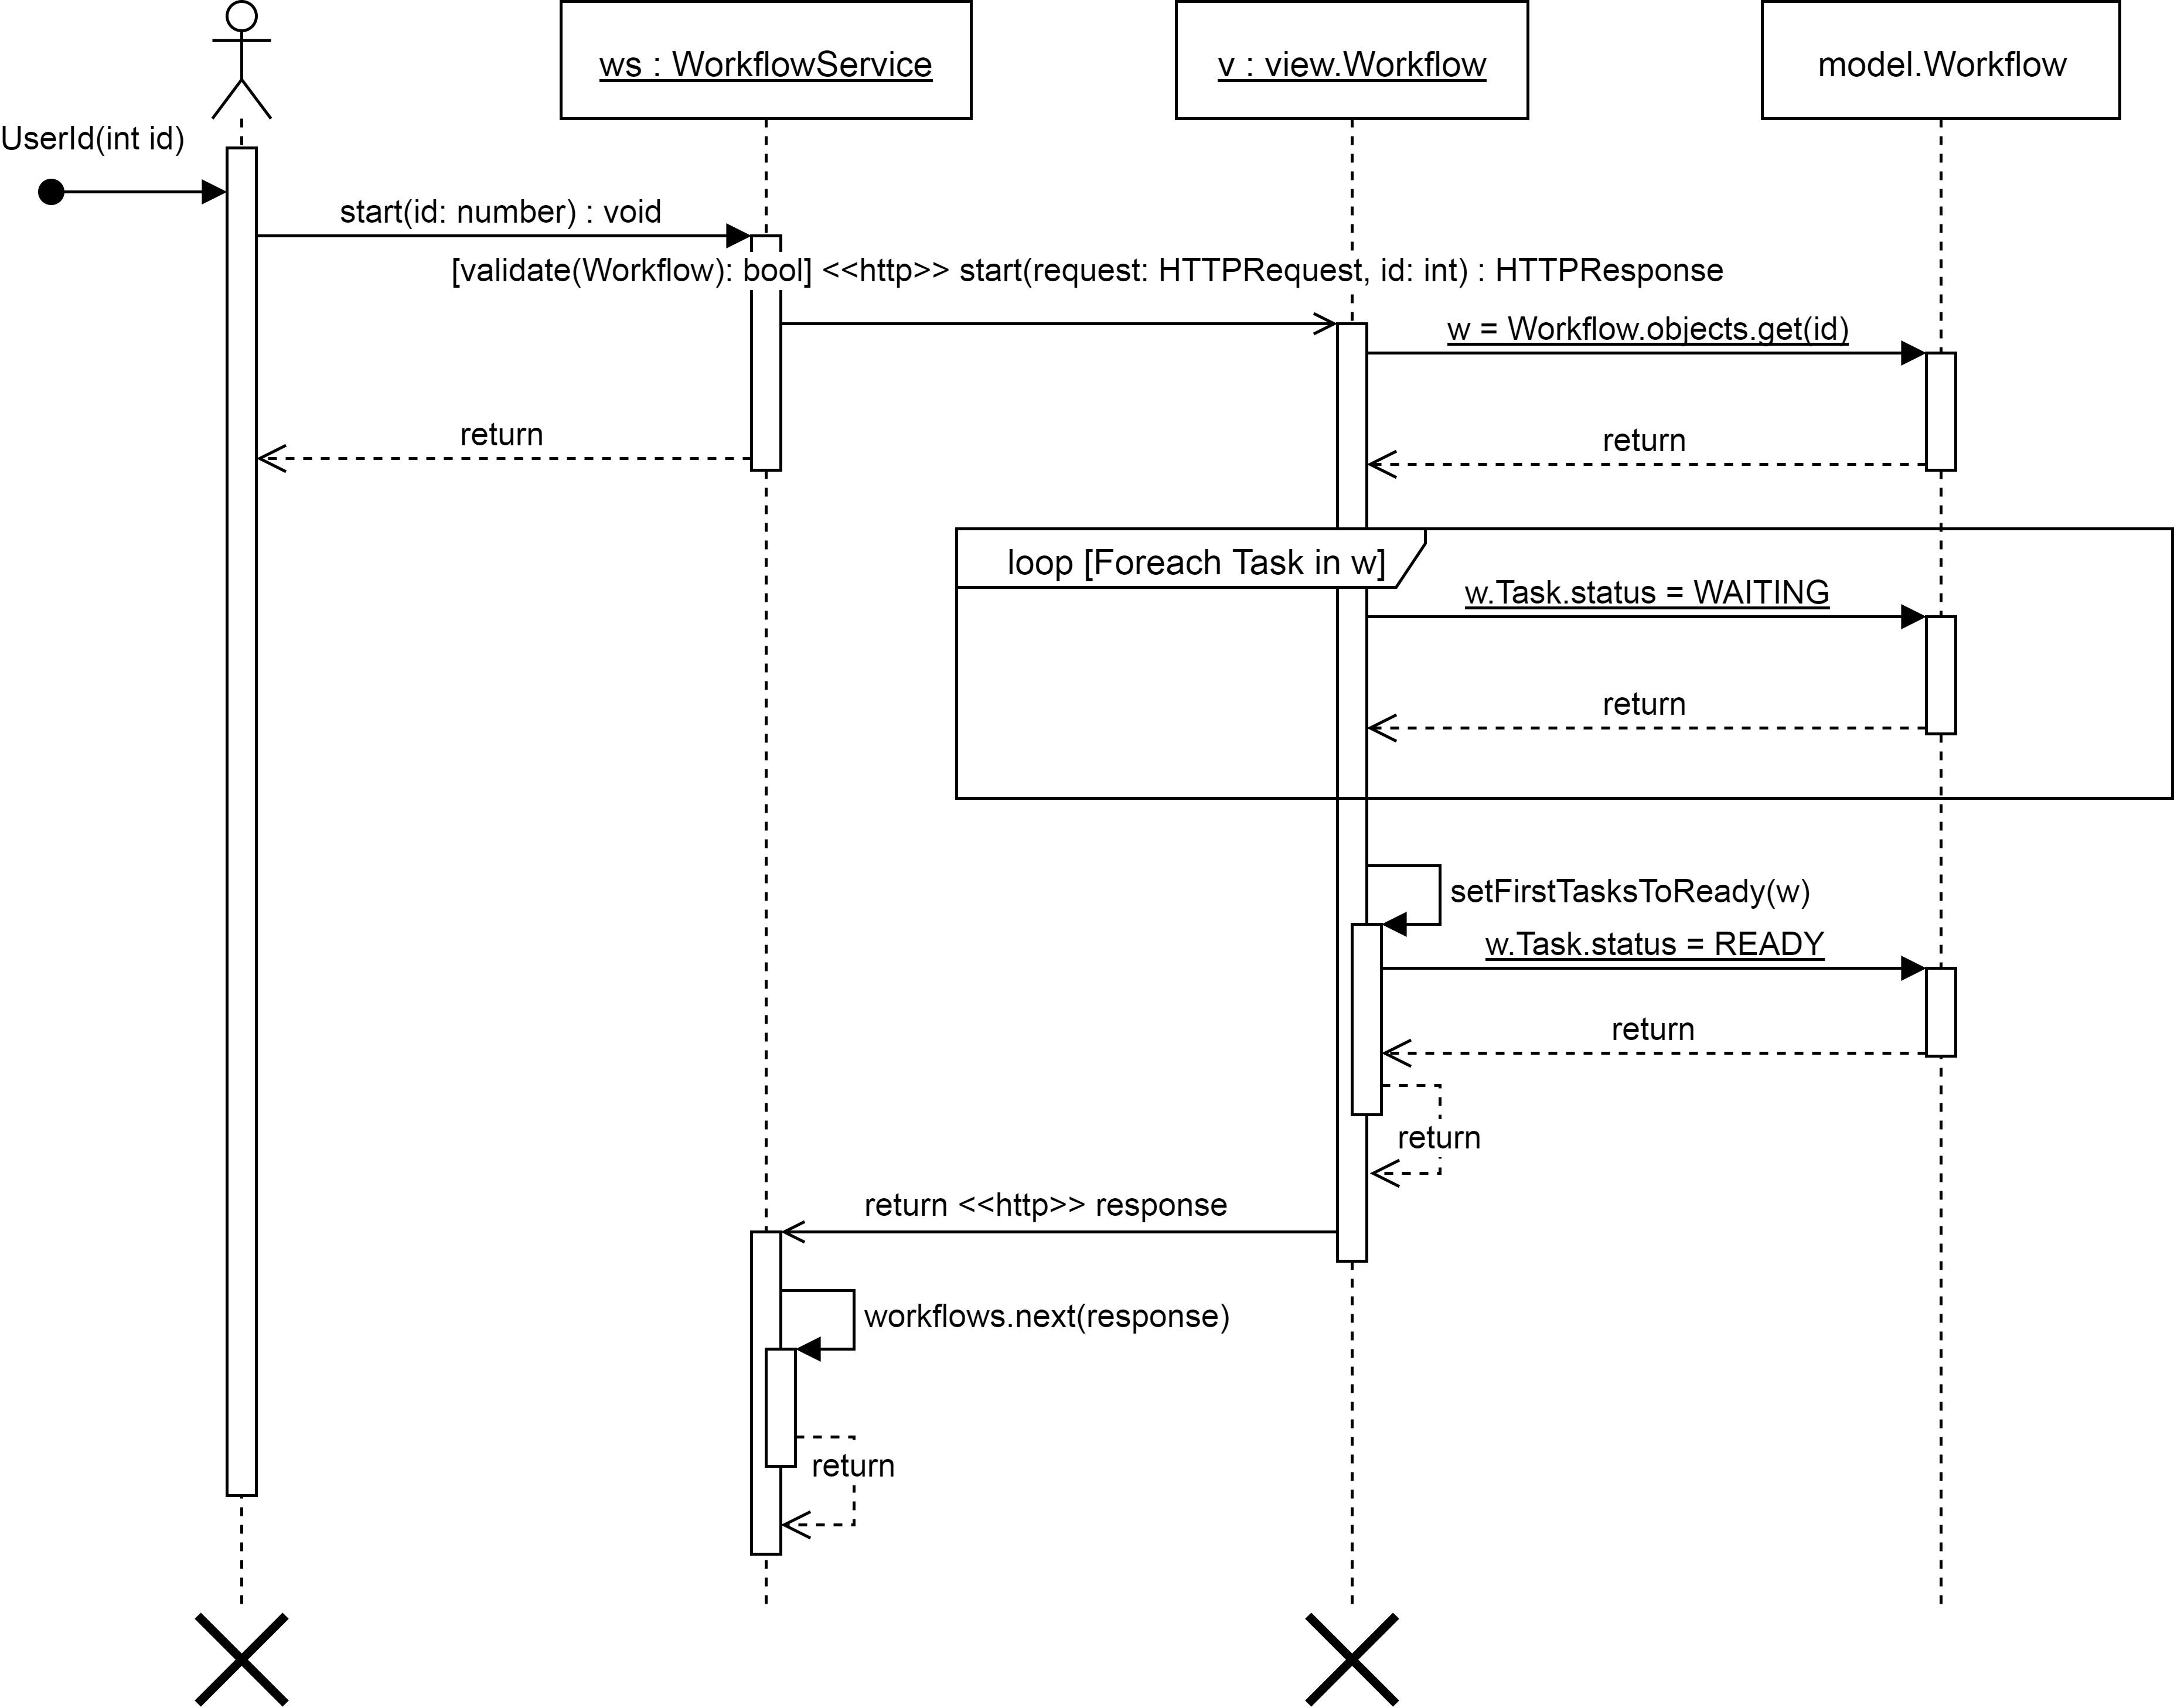
\includegraphics[width=15cm]{images/sqd_execute_workflow_client.jpg}
        \caption{Execute Workflow Clientside}
        \label{sqd_execute_workflow_client}
    \end{figure}
    
    \item Der Nutzer ist auch hier bereits angemeldet und hat einen Workflow geladen. Er beschließt den geladen Workflow auszuführen (Abbildung \ref{sqd_execute_workflow_client}). Hierfür wird an den WorkflowService start(id: int) geschickt, welcher mittels HTTP Request an view.Workflow weitergeleitet wird, vorausgesetzt, dass die Syntax korrekt ist. Serverseitig (view.Workflow) wird dann die aktuelle Version des Workflows aus der Datenbank geladen und der Status aller Tasks des Workflows auf \grqq{}WAITING\grqq{}  gesetzt. Danach werden die ersten, bzw. der erste Task ermittelt und dieser auf \grqq{}READY\grqq{}  gesetzt, damit diese(r) dann automatisch von Cron gestartet werden / wird. \newline\newline
    
    \begin{figure}[H]
        \centering
        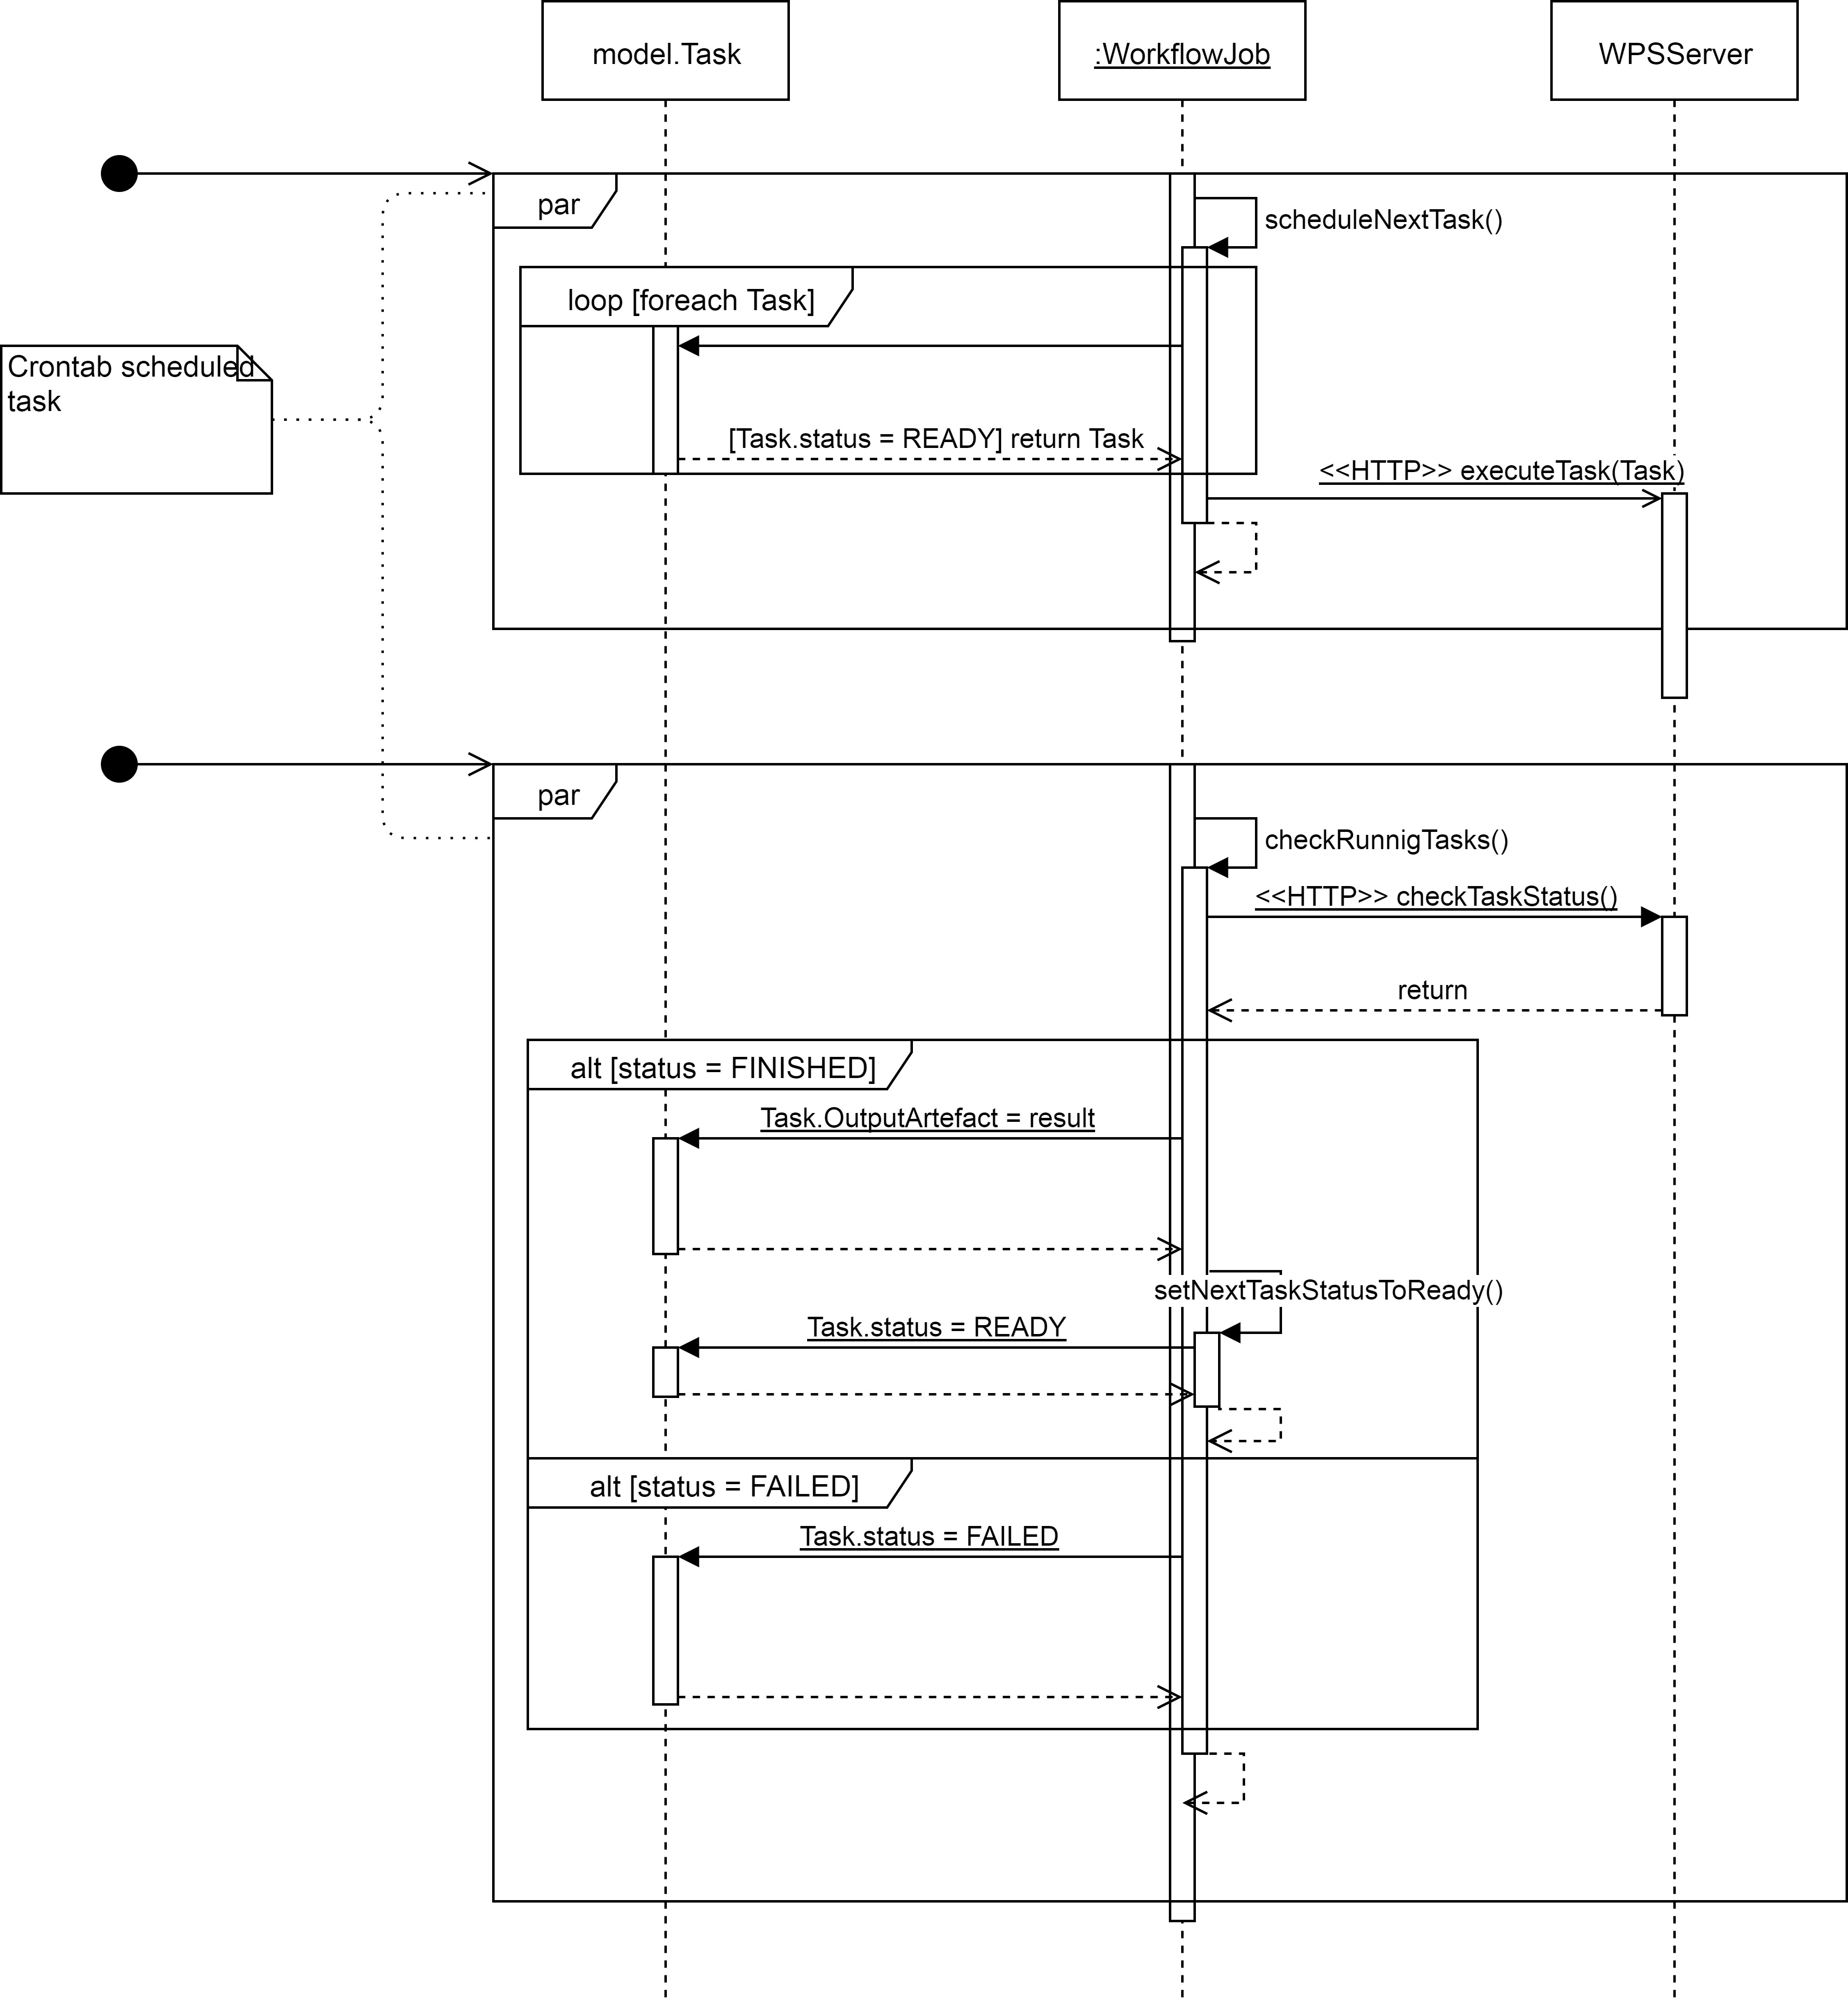
\includegraphics[width=15cm]{images/sqd_execute_workflow_server.jpg}
        \caption{Execute Workflow Serverside}
        \label{sqd_execute_workflow_server}
    \end{figure}
    
    \item Serverseitig werden mittels Crontab in WorkflowJob zwei Jobs parallel ausgeführt (Abbildung \ref{sqd_execute_workflow_server}). Der Job scheduleNextTask() lädt stets den nächsten Task, welcher \grqq{}READY\grqq{} ist von der Datenbank, und führt den Task asynchron auf dem entsprechenden WPS Server aus.
    \newline
    Der Job checkRunnigTasks() prüft regelmäßig alle Tasks, welche derzeit ausgeführt werden, ob sie bereits fertig sind. Wenn ein Task fertig ist werden die Ergebnisse in die Datenbank geladen und anschließend werden die darauf folgenden Tasks überprüft, ob sie alle Voraussetzungen erfüllen und ausgeführt werden können. Wenn dem so ist, wird deren Status von \grqq{}WAITING\grqq{}  auf \grqq{}READY\grqq{}  gesetzt, was dazu führt, dass der Job scheduleNext() sie ausführt. Wenn ein Task in einem Workflow fehlschlägt wir der Status des gesamten Workflows auf \grqq{}FAILED\grqq{} gesetzt, und die weiteren Tasks werden nicht ausgeführt.

\end{itemize}
